\chapter{Theoretical Overview}
\label{chap:Theory}

\section{Standard Model}
The Standard Model (SM) is a relativistic quantum field theory describing all known fundamental interactions between elementary particles with the exception of gravity, i.\,e. it describes electromagnetism as well as the weak and strong interactions. One has not yet succeeded integrating gravity into the same framework. However, since gravitational effects are negligible LHC energies, gravity can be safely ignored for our purposes.

The SM makes use of several types of fields, each describing a different kind of particle. The model contains half-integer and integer spin particles (in units of the reduced Planck constant $\hbar$) which are called fermions and bosons, respectively. Refs.~\cite{i2003gauge,aitchison2003gauge} elaborate on the individual types of particles in greater detail.\footnote{The present section as well as Sec.~\ref{sec:Theory/Shortcomings} are largely taken from Ref.~\cite{Thomassen2012} (the author's Master's Thesis).}

\begin{table}
	\centering
	\begin{tabular}{c||c|c|c|c}
		 & \textbf{particle} & $\begin{matrix}\textbf{mass} \\ \text{[MeV/$c^2$]}\end{matrix}$ & \textbf{spin} & $\begin{matrix}\textbf{electrical} \\ \textbf{charge} \text{ [$e$]}\end{matrix}$ \tabularnewline
		\hline 
		\hline 
		 & \multicolumn{4}{c}{} \tabularnewline
		 & \multicolumn{4}{c}{\textbf{fermions}} \tabularnewline
		\hline
		\multirow{6}{*}{$\begin{matrix}\textbf{leptons} \\ \\ L = 1, \\ B = 0\end{matrix}$} & $e$ & 0.511 & \nicefrac{1}{2} & $-1$ \tabularnewline
		 & $\nu_{e}$ & $0 < m_{\nu_e} < 2.2\cdot10^{-6}$ & \nicefrac{1}{2} & 0 \tabularnewline
		 & $\mu$ & 105.7 & \nicefrac{1}{2} & $-1$ \tabularnewline
		 & $\nu_{\mu}$ & $0 < m_{\nu_\mu} < 0.17$ & \nicefrac{1}{2} & 0 \tabularnewline
		 & $\tau$ & $1.78\cdot 10^3$ & \nicefrac{1}{2} & $-1$ \tabularnewline
		 & $\nu_{\tau}$ & $0 < m_{\nu_\tau} < 15.5\cdot10^{-6}$ & \nicefrac{1}{2} & 0 \tabularnewline
		\hline
		\multirow{6}{*}{$\begin{matrix}\textbf{quarks} \\ \\ L = 0, \\ B = \nicefrac{1}{3}\end{matrix}$} & $u$ & 2.4 & \nicefrac{1}{2} & $\nicefrac{2}{3}$ \tabularnewline
		 & $d$ & 4.8 & \nicefrac{1}{2} & $-\nicefrac{1}{3}$ \tabularnewline
		 & $c$ & $1.27\cdot 10^3$ & \nicefrac{1}{2} & $\nicefrac{2}{3}$ \tabularnewline
		 & $s$ & 104 & \nicefrac{1}{2} & $-\nicefrac{1}{3}$ \tabularnewline
		 & $t$ & $173.34 \cdot 10^3$ & \nicefrac{1}{2} & $\nicefrac{2}{3}$ \tabularnewline
		 & $b$ & $4.2\cdot 10^3$ & \nicefrac{1}{2} & $-\nicefrac{1}{3}$ \tabularnewline
		\hline
		 & \multicolumn{4}{c}{} \tabularnewline
		 & \multicolumn{4}{c}{\textbf{bosons}} \tabularnewline
		\hline
		\multirow{5}{*}{$\begin{matrix}L = 0, \\ B = 0\end{matrix}$} & $\gamma$ & 0 & 1 & 0 \tabularnewline
		 & $g$ & 0 & 1 & 0 \tabularnewline
		 & $Z$ & $91.2\cdot 10^3$ & 1 & 0 \tabularnewline
		 & $W^\pm$ & $80.4\cdot 10^3$ & 1 & $\pm 1$ \tabularnewline
		 & $H$ & $125.09 \cdot 10^3$ & 0 & 0 \tabularnewline
	\end{tabular}
	\caption{Elementary particles in the Standard Model \cite{PhysRevD.86.010001,ATLAS:2014wva,Aad:2015zhl}. For electrically charged particles, anti-particles with opposite charge exist. Neutrinos presumably have anti-particles with opposite chirality. Anti-particles have been omitted in this summary.}
	\label{tab:SM}
\end{table}

\subsection{Fermions}
The fermion group\footnote{``Group'' is not meant in the mathematical sense here.} consists of two subgroups named leptons and quarks; both of them are subdivided into three so-called ``generations'', or ``flavors''.

\subsubsection*{Leptons}
The three lepton generations are
\begin{eqnarray}
	\begin{pmatrix}\nu_e \\ e \end{pmatrix}, \quad
	\begin{pmatrix}\nu_\mu \\ \mu \end{pmatrix}, \quad
	\begin{pmatrix}\nu_\tau \\ \tau \end{pmatrix},
\end{eqnarray}
where $e$, $\mu$, $\tau$ are similar particles of electrical charge $-1$ and spin \nicefrac{1}{2}. However, their masses are quite different (see Table~\ref{tab:SM}). In interactions, they usually appear with the corresponding neutrino $\nu_\ell$, $\ell = e, \mu, \tau$. In addition to these six particles, there are also six antiparticles with opposite charge sign and lepton number.\footnote{It is also possible that neutrinos are Majorana fermions and thus their own anti-particles, as is the case in the type-III seesaw model, for example. This question has not yet been answered experimentally.} The present analysis is concerned with events exhibiting three or more electrons or muons.

\subsubsection*{Quarks}
There are six quarks called up, down, charm, strange, top, and bottom quark. They are organized in generations as follows:
\begin{eqnarray}
	\begin{pmatrix}u \\ d \end{pmatrix}, \quad
	\begin{pmatrix}c \\ s \end{pmatrix}, \quad
	\begin{pmatrix}t \\ b \end{pmatrix},
\end{eqnarray}
where the particles in the upper row are of electrical charge $+\nicefrac{2}{3}$, and those in the lower row have electrical charge $-\nicefrac{1}{3}$. Anti-quarks have opposite charge and baryon number. As quarks are subject to strong interaction, they carry an additional ``color'' charge which is either ``red'', ``green'', or ``blue''.

Quarks have not been observed individually. In the SM, they thus form bound states such that the electrical charge is integer and the color charge vanishes or adds up to ``white'' (i.\,e. all three colors are present). Particles consisting of three quarks are called baryons (for example the proton: $p \equates uud + \textrm{valence quarks}$), and quark--antiquark combinations are called mesons (for example the pion: $\pi^+ \equates u \bar d$).

\subsection{Bosons}
The quantum field theory on which the SM is built is invariant under Lorentz and CPT transformations, and under certain gauge transformations. To prevent the theory from losing this invariance, the existence of so-called gauge bosons was predicted, and indeed later observed. These particles act as the force carriers of the fundamental forces.

The most well-known one is the massless photon ($\gamma$) which is electrically neutral and mediates the electromagnetic interaction. A very similar particle, although massive, is the $Z$ boson which can interact electromagnetically and weakly. Furthermore, the charged $W^+$ and $W^-$ bosons exist. Conceptually, they have the same origin as the $Z$ boson, which is why they take part in the same interactions.\footnote{In fact, the $\gamma$ and $Z$ fields are superpositions of the more fundamental $B$ and $W^0$ fields. The $B$ field arises from spontaneous $U(1)$ symmetry breaking, while the $W^i$ come from the breaking of $SU(2)$.} A great theoretical achievement was the unification of the electromagnetic and the weak interaction into a combined concept, the electroweak interaction.

The strong force between quarks is carried by the massless gluons ($g$) which come in eight different color-anticolor combinations.

\section{Shortcomings of the Standard Model}
\label{sec:Theory/Shortcomings}

While the Standard Model predicts the electromagnetic, weak, and strong phenomena with extraordinary precision, there are open questions that are not addressed by the SM:
\begin{itemize}
	\item The Standard Model does not account for \textit{gravity} at all. It is described by General Relativity, and it is believed that, in principle, a unification of the theories is possible.
	\item The Standard Model contains a number of parameters that differ from expectation by several orders of magnitude for unknown reasons. For example, the mass of the Higgs boson was expected to be around $10^{15}\GeV$ due to top quark loops, but it is in fact on the electroweak scale \cite{Aad:2015zhl}. This issue is referred to as the \textit{Hierarchy Problem} \cite{Martin:1997ns}.
	\item The Standard Model does not explain \textit{Dark Matter} \cite{Pomarol:2012sb}.
	\item The Standard Model requires the neutrinos to be massless. However, the existence of oscillations between neutrinos flavors has been experimentally observed, implying that their mass is in fact non-zero \cite{PhysRevD.22.2227,Fukuda:1998fd,Nustatus}.
\end{itemize}

While the first three issues represent aspects of Nature that are not included in the SM or that remain puzzling, the neutrino mass issue is a serious problem, as the SM directly contradicts the experimental evidence \cite{Fukuda:1998fd}.

Several attempts have been made to find remedies for these issues from a theoretical point of view, and because they come with predictions of new particles, they are subject to experimental examination. The seesaw mechanism aims to provide answers to the question of how neutrinos acquire mass. 

\section{Type-III Seesaw Mechanism}
\subsection{Phenomenology}
\label{sec:Theory/SeesawPhenomenology}

The seesaw mechanism introduces new heavy particles coupling both to leptons and to Higgs doublets, and accounts for both the neutrino masses and their smallness (six or more orders of magnitude smaller than that of the electron) \cite{SeesawI,typeIa,typeIb,typeIe,typeIIa,typeIIb,typeIIc,typeIId,typeIIe,SeesawIII:a,Seesawinverse}.

%These new heavy particles could be weak-singlet fermions (type I \cite{SeesawI,typeIa,typeIb,typeIe}); weak-triplet scalars (type II \cite{typeIIa,typeIIb,typeIIc,typeIId,typeIIe}); or weak-triplet fermions (type III \cite{SeesawIII:a}). They generate a small Majorana mass for the neutrinos, given by, in type I and type III models: $m_{\nu}=Y^T~ \mathcal{M}^{-1}~ Y ~ v^2/2$, where $Y^T$ is the transpose of the Yukawa coupling matrix between the mediators and the SM fermions, $\mathcal{M}$ is the mass matrix of the heavy partner of the neutrinos and $~v$ is the Higgs vacuum expectation value. When mediator mass is large enough (of order of $10^{14}\GeV$), small neutrino masses are generated even for order $O(1)$ Yukawa couplings. If $M$ is smaller (of the order of a few hundreds of \GeV, as in LHC searches), either smaller Yukawa couplings (i.\,e. ``natural'' mixing angles of the order of $10^{-6}$) are required to generate small neutrino masses, or an alternative suppression mechanism is needed (e.\,g. seesaw inverse mechanism \cite{Seesawinverse}). The possible allowed values of the mixing parameters and their products are constrained by precision electroweak data \cite{typeIIIconstraint}.

Within the type-III seesaw model \cite{SeesawIII:a}, the neutrino is considered a Majorana particle whose mass arises via the mediation of massive fermion partners. These massive partners are the fermionic $SU(2)$ triplet of the heavy Dirac charged leptons $\Sigma^\pm$, and the heavy Majorana neutral lepton $\Sigma^0$, coupling both to the leptons and to the Higgs doublets. During proton-proton collisions, the heavy fermion particles may be pair-produced through electroweak interactions in both charged-charged and charged-neutral pairs as can be seen in Fig.~\ref{fig:SeesawProduction}.

\begin{figure}
\begin{center}
	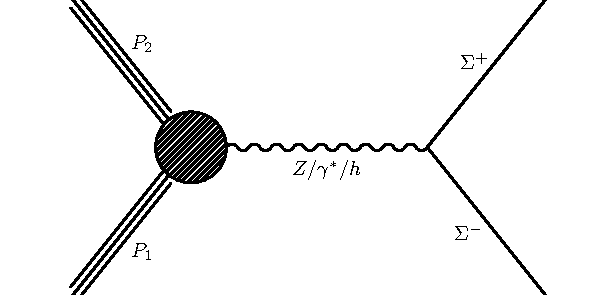
\includegraphics[width=.5\textwidth]{Introduction/SeesawProduction-SpSm}%
	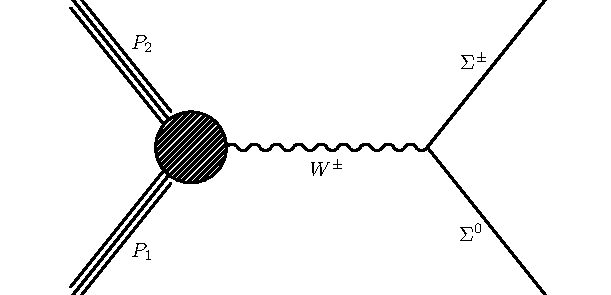
\includegraphics[width=.5\textwidth]{Introduction/SeesawProduction-SpmS0}
	\caption{Examples of Feynman diagrams for heavy fermion production in the type-III seesaw model.
	\label{fig:SeesawProduction}}
\end{center}
\end{figure}

We conduct a search for this signal by examining the final state with at least three electrons or muons. The primary decay channels of interest are $\Sigma^\pm \to \PW^\pm \nu$, $\Sigma^\pm \to \Z \ell^\pm$, $\Sigma^\pm \to \PH \ell^\pm$, $\Sigma^0 \to \PW^\pm \ell^\mp$, $\Sigma^0 \to \Z \nu$, $\Sigma^0 \to \PH \nu$, where $\ell = e, \mu$. Decays of $\Sigma^0 \Sigma^\pm$ and $\Sigma^+ \Sigma^-$ pairs result in 27 different production processes and can naturally lead to multilepton final states if several \PW\ or \Z\ bosons are involved, either directly or via a Higgs boson decay. An example Feynman diagram for one of the most relevant processes with three leptons in the final state, $\Sigma^\pm \Sigma^0 \to \PW^\pm \nu \PW^\pm \ell^\mp$ with leptonic $\PW^\pm$ decays, is shown in Fig.~\ref{fig:SeesawDecay}.
The decay rate of a $\Sigma$ to a given lepton $\ell$ is proportional to $v_{\ell N} = \frac{V_\ell}{\sqrt{|V_e|^2 + |V_\mu|^2 + |V_\tau|^2}}$. In the democratic scenario, the mixing parameters $V_\ell$ are the same for all the leptons.

\begin{figure}
\begin{center}
	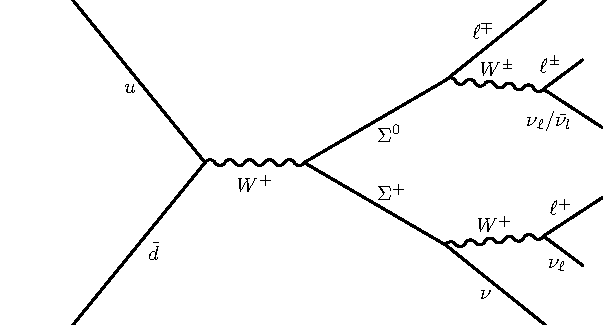
\includegraphics[width=.5\textwidth]{Introduction/Seesaw}
	\caption{Feynman diagram example of the fermion production and decay in the type-III seesaw model.
	\label{fig:SeesawDecay}}
\end{center}
\end{figure}


\subsection{Signal Model and Generation}
\label{sec:Samples/Signal}

We generate MC events to simulate all 27 production and decay mode combinations (see Sec.~\ref{sec:Introduction}). Generation for the model begins with a FeynRules Model file \cite{SeesawIII_Biggio}. SaloMonte Carlo events are then generated in MadGraph5\_aMC@NLO \cite{Alwall:2011uj}. Bosonic decays are handled through Pythia 8, which is also in charge of hadronization \cite{Sjostrand:2007gs}. At the analysis level, we apply weights to correct for mismodeling of pile-up and \MET resolution.

The production cross sections were calculated with NLO + NLL accuracy using the CTEQ6.6 and MSTW2008nlo90cl parton distribution functions (PDFs) \cite{Fuks:2012qx,Fuks:2013vua}. Flavor-democratic values of the mixing angles are taken ($V_e = V_\mu = V_\tau = 10^{-6}$). This has no direct consequence on the fermion production cross section, but affects the branching ratios. The branching fraction of a heavy fermion to a lepton of flavor $\ell = e, \mu, \tau$ is proportional to $v_{\ell N} = \frac{V_\ell}{\sqrt{|V_e|^2 + |V_\mu|^2 + |V_\tau|^2}}$. Therefore, the flavor-democratic scenario gives $v_{\ell N} = \frac{1}{\sqrt{3}}$. The branching ratios from the pair-produced fermions to the bosonic level of the most relevant decay modes are given in Fig.~\ref{fig:SeesawBR}.

\begin{figure}
\begin{center}
	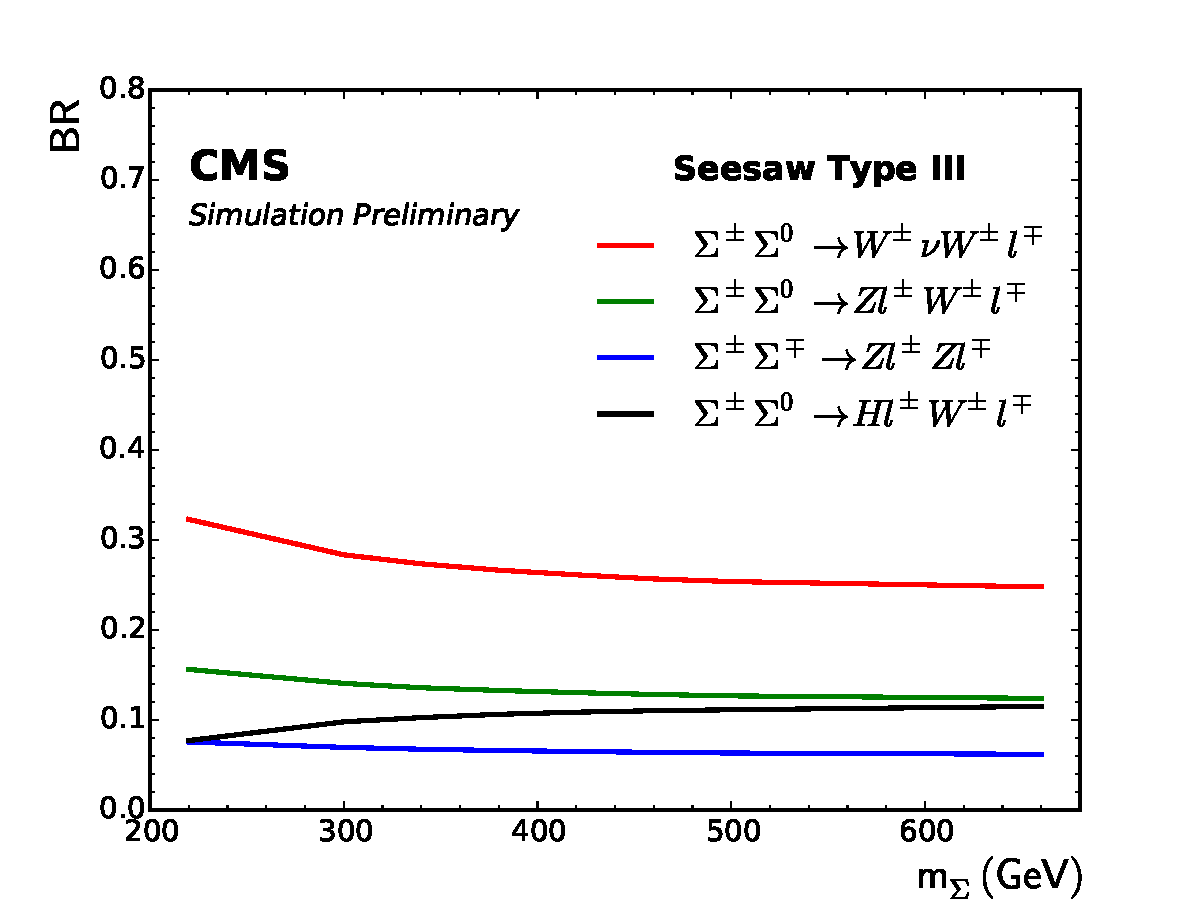
\includegraphics[width=.8\textwidth]{Theory/BR}
	\caption{Branching ratios from the pair-produced fermions to the bosonic level of the most relevant decay modes.
	\label{fig:SeesawBR}}
\end{center}
\end{figure}
